\subsection{Mechanism Construction}
\label{sec:generator-expression-pipeline}

\citet[Section~2.1]{dascoli2022deep} generate recurrent-sequence examples by
sampling an expression tree, selecting initial conditions, and executing the
recurrence. The implementation adopts this expression-first organization and
retains separate representations of structure and numerical values, as
defined in Section~\ref{sec:generator-vocabulary}. A user-provided equation
and a sampled expression can therefore enter the same execution pipeline.

\begin{figure}[H]
\centering
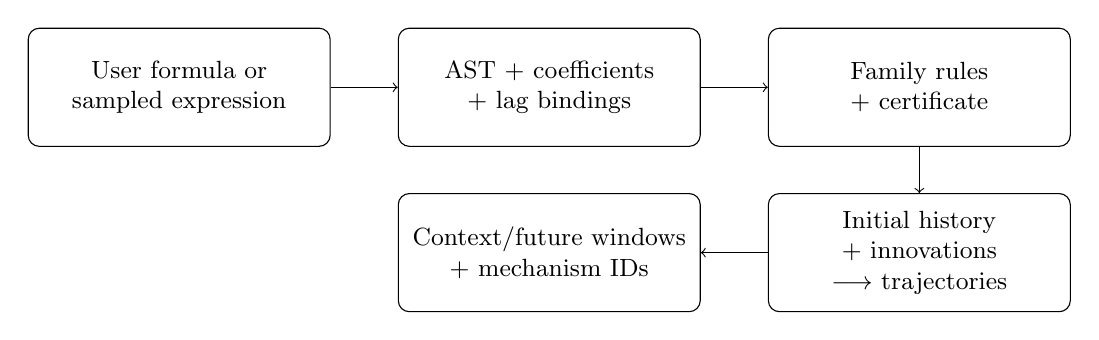
\begin{tikzpicture}[box/.style={draw,rounded corners,align=center,
    text width=3.6cm,minimum height=1.5cm,font=\small}]
\node[box] (tree) at (0,0) {User formula or\\sampled expression};
\node[box] (bound) at (4.7,0) {AST + coefficients\\+ lag bindings};
\node[box] (family) at (9.4,0) {Family rules\\+ certificate};
\node[box] (paths) at (9.4,-2.1) {Initial history\\+ innovations\\$\longrightarrow$ trajectories};
\node[box] (batch) at (4.7,-2.1) {Context/future windows\\+ mechanism IDs};
\draw[->] (tree) -- (bound);
\draw[->] (bound) -- (family);
\draw[->] (family) -- (paths);
\draw[->] (paths) -- (batch);
\end{tikzpicture}
\caption{Implemented generation stages. The selected family determines the
admissible expressions, initialization, and innovation law. The mechanism
record is retained alongside the observations.}
\label{fig:implemented-generator-pipeline}
\end{figure}

\subsubsection{Random Tree Sampling}
Within the selected vocabulary in Section~\ref{sec:generator-vocabulary},
the base sampler draws a binary-operator count, labels leaves as parameters
or lagged series, and recursively constructs the tree. Its implementation
is in \path{src/tsfmxai/generators/random_expression.py}.
For a subtree containing $o$ binary operators, the
probability of assigning $a$ operators to the left child is proportional to
the number of left shapes times the number of right shapes. These counts
are Catalan numbers. This produces a uniform distribution over ordered full
binary shapes conditional on $o$. Internal nodes
are labelled addition or multiplication. Zero-operator trees consist of one
leaf; required leaf types must fit the requested size.

The current random base grammar therefore uses binary operations; the
Shao--Wu transformation in Section~\ref{sec:implemented-shao-wu}
adds unary \texttt{Tanh} nodes to the same AST
representation. The wider unary--binary grammar in D'Ascoli et al.
provides the precedent. Our operator probabilities, parameter ranges, forced
lag presence, and multivariate source indices define the project's sampling
prior. Slot names are assigned in preorder, preserving the sampled left and
right children. This keeps numerical bindings and serialization reproducible
for a fixed seed.

\subsubsection{User-Provided Equations}
A researcher can specify the expression structure and its bindings directly
within the vocabulary in Section~\ref{sec:generator-vocabulary}. For example,
the skeleton $P_0x_0(t-L_0)+P_1$ becomes
$0.7x_0(t-2)+0.01$ after binding its slots. Numerical parameters and lag
assignments are retained with the AST so the resulting formula is executable
and can be inspected independently of its generated observations.
The selected family then applies its construction and admissibility rules
as described in Section~\ref{sec:generator-stability}; the resulting,
possibly transformed equation is the mechanism used for execution and
ground-truth extraction.
